% !TeX root = ../thuthesis-example.tex

\chapter{集群故障检测和判断}

集群故障检测和判断是构建高可用自动容错能力的先决条件。如同医生诊断病情是进行治疗的第一步,系统也必须先感知到问题的存在,才能采取相应的应对措施。及时、准确地识别出集群中发生的各种故障,是后续所有容错机制得以有效运行的前提。

本章节描述了高可用框架下的集群故障检测和判断机制。管理节点是集群的大脑,负责集群故障检测和研判。管理节点通过和集群所有成员交换心跳定期收集信息,并使用集群故障研判的算法来发现故障。

本节描述了管理节点、数据节点和客户端之间通过心跳探知其他节点状态的机制,并描述了基于心跳历史的固定超时、Phi Accrual算法的故障研判机制。


\section{不同角色的状态感知机制}

\subsection{管理节点感知其他节点状态}

管理节点节点通过共识心跳感知其他管理节点的状态,通过定期的心跳RPC感知所有数据节点的状态。

管理节点 集群通过 Raft 协议中领导者定期发送的心跳以及 Follower 基于这些心跳维护的选举超时计时器,实现了对集群中其他管理节点的成员列表、每个成员的基本存活状态的高效感知。一旦心跳机制指示领导者节点失联或故障,就会触发 Raft 的选举流程,确保管理节点集群在面对节点失效时能够及时地重新组织并恢复正常工作。

IoTDB通过管理节点和数据节点定期交换心跳的机制来维护每一个数据节点节点的信息,并用这些信息进行磁盘、进程和对称网络分区的故障探测。管理节点和数据节点之间心跳交换的具体实现如下。

管理节点会将集群的所有数据节点纳入心跳管理的范畴。具体来说,数据节点在启动时都需要向管理节点的领导者节点汇报和注册自己。一经注册,管理节点领导者就会将这个进程纳入到心跳管理的范围内。同样,在节点下线维护、被移出集群、重启时也会向管理节点进行汇报,由管理节点决定是否要将节点移除出心跳管理的范畴。

对于纳入心跳管理范畴的节点,管理节点会按照固定时间间隔(默认为1s)向这些节点的内部端口发送RPC心跳探测,并要求节点上传自身的信息,确认最新的状态。以数据节点为例,数据节点需要通过心跳上报当前的存活状态、节点的CPU负载率、内存占用率、磁盘的消耗情况以及数据节点上每一个分区的情况,包括分区领导者的身份确认、每一个分区的磁盘占用情况、副本日志同步的情况、数据节点上所有pipe任务的情况。

通过定期交换信息,管理节点能够掌握节点的全局信息,并利用上述这些信息展开对磁盘写满、节点宕机、网络对称分区等错误的检测。具体的检测方法可以参考后续的章节\ref{failure_detection}。

\subsection{数据节点感知其他节点状态}\label{sec:数据节点-intra-heartbeat}

通过和管理节点交换心跳,数据节点能够实时感知管理节点的列表和存活状态。

为了让数据节点能够实时感知其他数据节点成员的状态,本文提出基于数据节点间的对等心跳汇总的集群拓扑感知机制,通过数据节点之间定期交换心跳来获取相互之间的连通性,并将所有节点的结果汇总上报给管理节点领导者,从而使管理节点领导者具备集群的网络拓扑感知能力。

\begin{figure}
  \centering
  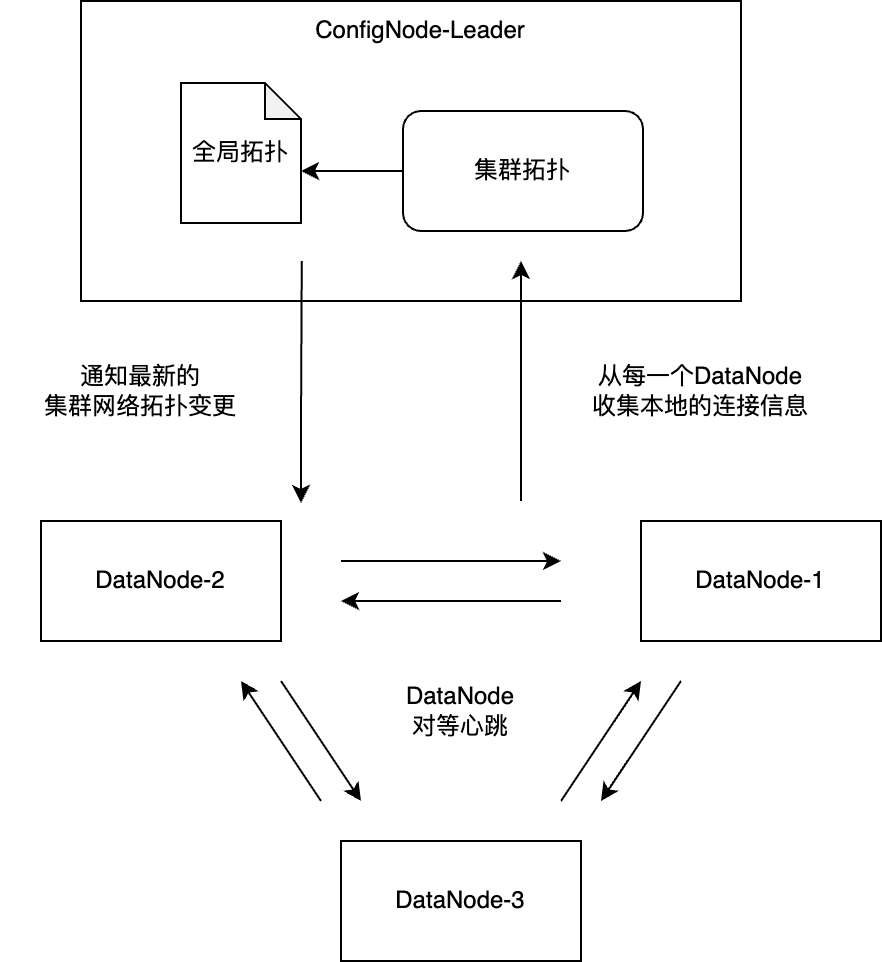
\includegraphics[width=0.8\linewidth]{c03-topology-redraw.png}
  \caption{集群拓扑感知能力}
  \label{fig:c03-topology}
\end{figure}

图\ref{fig:c03-topology}给出了数据节点间的对等心跳机制描述。

管理节点会定期要求集群中的每个数据节点都与其他数据节点进行对等的心跳交换。通过这种全互联的心跳机制,每个数据节点能够更直接地获取自己与其他数据节点性状态,例如是否能够成功发送心跳、是否能够及时收到对方的心跳响应等。

随后,每个数据节点会将自己收集到的与其他数据节点的连通性信息进行汇总和整理,形成一个局部的网络拓扑视图。这个视图包含了该数据节点对集群中其他数据节点可达性的判断。

为了获得全局的视角,每个数据节点会将这个汇总后的连通性报告定期地上报给当前的管理节点领导者。管理节点领导者作为集群的中央协调者,在接收到来自所有数据节点的连通性报告后,便能够汇总所有节点的局部视图,从而构建出一个完整的、全局的集群网络拓扑感知能力。与仅仅依赖管理节点和数据节点之间的单向心跳相比,这种方式能够更全面地了解集群内部节点之间的双向通信状况。

在获取了全局视角的网络拓扑图之后,管理节点会通过RPC的方式将这个全局拓扑下放通知给所有的数据节点,从而赋予每一个数据节点更加完善的集群状态感知能力,允许在后续的写入规划、查询规划等操作更加智能、可靠。

\subsection{客户端节点感知其他节点状态}

客户端会对集群的数据节点状态有所感知,这个感知是两阶段的过程,首先,它依赖于从管理节点获取最新的、潜在可用的数据节点列表及其地址;然后,它通过主动尝试与目标数据节点建立连接来直接验证该数据节点在客户端视角下的实际可达性和存活状态。

客户端并不会预先硬编码所有可能的数据节点地址。相反,客户端在初始化或需要更新集群视图时,会首先与管理节点集群建立连接。管理节点 集群作为整个 IoTDB 分布式系统的元数据管理者,维护着最新的集群拓扑信息,包括当前注册在集群中的所有数据节点的网络地址。

客户端通过后台线程定期(通常是60s)向管理节点拉取当前管理节点认为活跃或已知的数据节点列表及其对应的通信地址。

获取到数据节点列表后,客户端并不会向所有数据节点发送请求。当客户端需要与某个特定的数据节点进行交互时,客户端会尝试与该数据节点的网络地址建立Thrift连接并发送交互请求。如果请求成功,那么客户端会认为该节点存活状态良好。反之,客户端会判断该节点当前不可用。

\section{基于状态感知的故障检测算法}\label{failure_detection}

\subsection{固定心跳超时判断}\label{failure_detection_timeout_fix}

在本文的工作之前,IoTDB内部采用基于心跳固定超时时间的故障检测。该算法可以概括为,如果节点在超过一段时间之后没有收到另外一个节点的心跳,那么就会认为另外的这个节点出现了故障,可能是网络分区或者进程宕机。
更具体地,我们定义超时时间参数$\Delta_{t}$(默认为20s),该参数的含义是:当管理节点领导者在超过$\Delta_{t}$的时间里面没有收到某一个被询问方数据节点的心跳,或者发起方数据节点在超过$\Delta_{t}$的时间里没有收到另外的一个被询问方数据节点的心跳,就会判断被询问方的数据节点不可达,可能是出现了网络分区或者其他问题。

这种基于心跳的固定超时算法的优点在于逻辑简单直接,易于实现和部署,并且在IoTDB已有的实践中能胜任大部分的错误发现。然而这种算法依然存在诸多问题,例如:

1. 固定的算法无法应对复杂和变化的系统环境。节点的网络变化、系统的负载变化、长时间的GC等诸多因素都有可能导致心跳包被延迟传输或拥塞,从而出现超时产生误判,触发不必要的容错操作。

2. 选择一个$\Delta_{t}$ 的最佳参数在实践中非常困难。一方面,参数的选择需要人工介入,需要用户对自身业务集群的特性、IoTDB内核的故障检测机制都有所了解,这对很多用户来说是一个很大的心智负担。
另一方面,参数 $\Delta_{t}$ 本身就是故障检测的检测速度和检测正确度的权衡。选择一个较短的$\Delta_{t}$参数,那么节点故障会被快速发现,但对应的误报率就会很高;如果选择一个较长的$\Delta_{t}$,虽然误报率会对应下降,但是错误的平均发现时间将会变长。

\subsection{Phi Accrual算法判断}

章节\ref{sec:cassandra-failure-detecttion}提到的Phi Accrual能够良好解决上述的两个问题。然而,Phi Accrual算法存在冷启动的问题。在节点启动、重启的阶段,如果错误地将节点判断成不可达,那么可能会导致不必要的\failover 、节点延迟加入集群或提供服务和增加运维复杂性等问题。

为此,本文最后提出的IoTDB故障研判算法是结合心跳固定超时时间的判断和Phi Accrual算法的结果。具体来说,IoTDB的故障检测将会根据节点的生命周期划分为两个阶段:冷启动阶段和正常服务阶段。

冷启动阶段。当节点刚刚启动,或是刚刚从故障恢复,此时我们尚未收集到足够的心跳样本,我们将会使用\ref{failure_detection_timeout_fix}提到的算法来负责初始时期的节点故障检测,并同时在后台继续收集样本。当我们收集了足够的样本数量(默认为60个)的时候,我们切换成基于Phi Accrual的算法来研判节点的存活率。由于节点在刚启动过程中往往不会立马承担较大的流量负载,也不太可能会发生长时间的垃圾回收等异常情况,因此在这个阶段使用固定超时算法将能较为有效地实现故障检测。

节点正常服务阶段。当节点稳定提供服务一段时间之后,我们已经收集到了足够的心跳历史样本,IoTDB集群将会切换为基于Phi Accrual的检测算法进行故障研判。具体的实现如下:

1. 收集心跳历史采样。对于每一个新到达的心跳包,算法会计算出和上一个心跳包之间的间隔,并将这个间隔存入一个固定大小(默认为100)的采样窗口内。当有新的心跳不断到达的时候,最新的一个间隔会被存入采样窗口,窗口最早的第一个间隔则会被剔除,以便更好地反映集群的近况。

2. 根据采样窗口计算到达间隔的分布,计算 $\phi$ 值。在Phi Accrual算法中, $\phi$ 值代表了一个节点出现故障的怀疑概率。
我们假设心跳到达间隔的分布符合正态分布,那么可以通过历史采样窗口来估计分布的均值 $\mu$ 和方差 $\sigma^2$。那么,在上一次心跳到达t时间之后才会有下一次心跳到达的概率可以通过下列公式计算出来:

$$ P_{later}(t) = \frac{1}{\sigma\sqrt{2\pi}} \int_{t}^{\infty} e^{-\frac{(x-u)^2}{2\sigma^2}} dx $$

在实际实现中,我们通过逻辑斯蒂分布对高斯分布进行近似\cite{bronvstejn2013handbook}:

$$ P_{later}(t) = \exp(1.5976 + 0.070566 (\frac{t-u}{\sigma})^2) $$

3. 计算 $\phi$ 并根据设定阈值进行比较。我们使用如下的公式进行定义:

$$ \phi(now) = -log_{10}(P_{later}(t_{now} - t_{last})) $$

用户可以通过设定不同的$\phi$阈值来控制研判的精准度。阈值越高,研判的精准度越高。在章节\ref{sec-experience-phi-accrual}中,我们给出了这个故障检测算法的实验验证和不同阈值参数下算法的表现行为。


\subsection{Thrift连接状态判断}\label{thrift-detection}

在\ref{failure_detection}中提到的故障研判,通过对心跳行为建立概率模型来判断节点是否发生故障。这种故障研判需要一定的观察窗口才能作出可靠的判断,因此发现故障通常需要十秒或者更久。

然而,在进程宕机、被系统强制关闭等特殊场景下,我们可以利用Thrift 长连接的特点,将被动的故障发现转化为主动的故障通知,从而显著加快故障的发现和传播速度。

IoTDB内部采用Thrift\cite{slee2007thrift}框架作为RPC通信的实现。Thrift框架底层使用网络协议层的TCP协议或者UDP协议实现实际的传输。IoTDB 内部采用 ClientManager 接口来统一管理对外的 Thrift 连接。ClientManager 的基本原理类似于带缓存的连接池。当我们首次请求连接到某一个新的 EndPoint(代表一个特定的 IP 地址和端口)时,ClientManager 会建立一个底层的 TCP 连接。与使用完毕后立即断开连接不同,ClientManager 会在结束使用后继续维持这个 TCP 连接一段时间,并将其缓存在本地。这样,在下次我们需要请求相同的 EndPoint 地址时,就不需要重新进行 TCP 三次握手等连接建立的开销,可以直接复用 ClientManager 内部缓存的现有连接。只有当某个 TCP 连接长时间没有被使用时,ClientManager 才会主动销毁该连接并清理相关的系统资源。

由于管理节点和每一个数据节点之间存在持续频繁的内部 RPC 通信,通过上述所言的 ClientManager 的机制,我们可以认为在管理节点和数据节点之间建立了一条长期有效的 TCP 连接信道,并在这个 TCP 信道的基础上建立了一个长期有效的 Thrift 连接。

Thrift框架能够感知其底层的TCP传输层的连接状态。当连接的进程突然出现故障,无论是是由于程序崩溃,还是被操作系统强制终止(例如使用 kill -9 命令),该进程所建立的TCP连接也会中断。
Thrift 能够迅速检测到这个信道的问题,并向上层的IoTDB模块汇报连接中断的事件。
这种主动汇报机制的时间延迟通常在故障发生的毫秒到秒级,非常快速。

管理节点领导者会利用这样的机制,在收到断开汇报的时候将该进程标记为失效,从而实现进程失效的快速检测和优化。

\section{本章小结}

本章详细阐述了 Apache IoTDB 分布式集群高可用与容错框架的集群故障检测和判断机制部分。及时、准确地感知故障是系统能够实施有效恢复和转移策略的前提。

章节首先描述了不同角色节点间的状态感知方式。


管理节点 作为集群的“大脑”,通过与管理节点之间基于 Raft 协议的心跳以及与数据节点之间定期的 RPC 心跳,周期性地收集集群各成员的基本存活状态、资源负载等信息。同时,数据节点之间也通过对等心跳进行连通性探测,并将结果上报给管理节点,增强了集群对内部网络状况的感知能力。客户端客户端则通过尝试建立和维持与数据节点的连接来判断其可达性。

在此状态感知的基础上,本章着重探讨了用于研判节点故障的算法。章节回顾了传统固定心跳超时算法的优缺点,指出其在复杂多变网络环境下易产生误判且参数难以调优的问题。进而引入并详细阐述了更具适应性的 Phi Accrual 算法,该算法通过分析心跳历史,以概率形式(Φ 值)判断节点的怀疑度,能够更精确地反映节点存活状态。考虑到 Phi Accrual 算法在冷启动阶段的不足,本章提出了一种结合策略:在节点冷启动阶段采用固定超时判断快速发现早期问题,在进入正常服务阶段后切换至基于 Phi Accuarl 算法进行更鲁棒的故障研判。